\documentclass[letterpaper,11pt]{scrartcl}

\setlength{\pdfpagewidth}{8.5in}
\setlength{\pdfpageheight}{11in}
\usepackage[T1]{fontenc}
\usepackage[utf8]{inputenc}
\usepackage{lmodern}
\usepackage{amsfonts,amsmath,amssymb,amsthm,mathtools}
\usepackage[letterpaper,margin=1in]{geometry}
\usepackage[english]{babel}
\setlength{\parindent}{1pt}
\setlength{\parskip}{0.75em}

% Venue-neutral author packages adapted from the ITBound v2 skeleton.
\usepackage{wrapfig}
\usepackage{mdframed}
\usepackage[authoryear,round]{natbib}
\usepackage{bm}
\usepackage{multirow}
\usepackage{array}
\usepackage{verbatim}
\usepackage[normalem]{ulem}
\usepackage{thmtools}
\usepackage{setspace}
\usepackage{adjustbox}
\usepackage{graphicx}
\usepackage{subfig}
\usepackage[useregional]{datetime2}
\usepackage{enumitem}
\usepackage[most]{tcolorbox}
\tcbuselibrary{theorems}
\usepackage{longtable}
\usepackage{ltablex}
\usepackage{nccmath}
\usepackage{sansmath}
\usepackage{booktabs,tabularx}
\usepackage{makecell}
\usepackage[dvipsnames]{xcolor}
\usepackage[colorlinks=true,citecolor=NavyBlue,linkcolor=RoyalBlue,urlcolor=NavyBlue]{hyperref}

\newtheorem{definition}{Definition}
\newtheorem{theorem}{Theorem}
\newtheorem{assumption}{Assumption}
\newtheorem{example}{Example}
\newtheorem{lemma}{Lemma}
\newtheorem{proposition}{Proposition}
\newtheorem{corollary}{Corollary}
\newtheorem{remark}{Remark}

\tcolorboxenvironment{definition}{colback=gray!5!white,colframe=black,fonttitle=\bfseries,boxrule=0.5pt,breakable}
\tcolorboxenvironment{theorem}{colback=gray!5!white,colframe=black,fonttitle=\bfseries,boxrule=0.5pt,breakable}
\tcolorboxenvironment{corollary}{colback=gray!5!white,colframe=black,fonttitle=\bfseries,boxrule=0.5pt,breakable}
\tcolorboxenvironment{lemma}{colback=gray!5!white,colframe=black,fonttitle=\bfseries,boxrule=0.5pt,breakable}
\tcolorboxenvironment{proposition}{colback=gray!5!white,colframe=black,fonttitle=\bfseries,boxrule=0.5pt,breakable}
\tcolorboxenvironment{remark}{colback=gray!5!white,colframe=black,fonttitle=\bfseries,boxrule=0.5pt,breakable}
\tcolorboxenvironment{assumption}{colback=white,colframe=black,fonttitle=\bfseries,boxrule=0.5pt,breakable}


\title{Proximal Balancing}
\author{Yonghan Jung}
\date{}

\begin{document}
\maketitle
\allowdisplaybreaks

\begin{abstract}
\emergencystretch=2em
We study causal adjustment with observed pretreatment covariates $X$, one pretreatment proxy $W$, and an unobserved confounder. In the canonical regime, $W$ supervises a finite representation $Z=\phi(X)$ but is not included in the final adjustment variable. We establish an exact bias decomposition and show that, under a uniform outcome-relevant stability condition, the observable residual imbalance $D(\phi)$ yields the sensitivity certificate $|\tau_\phi-\tau|\le\Gamma D(\phi)$. Exact balance identifies the average treatment effect under the stated proxy conditions, while a finite-class learning analysis controls the certificate achieved by empirical representation selection. We separately study a proxy-augmented audit-view construction that prevents literal self-conditioning; its point-identification result requires additional multi-view structure and remains a conditional extension. Accordingly, we do not claim that one generic proxy alone point-identifies the average treatment effect.

\end{abstract}

\tableofcontents
\newpage

\begingroup
\allowdisplaybreaks
\sloppy
\section{Introduction}
\label{sec:introduction}

\subsection{Related Works}
\label{sec:related-work}

\textbf{Balancing scores and covariate balancing.} The propensity score is the canonical reduction of observed pretreatment covariates: under treatment ignorability given $X$, conditioning on $e(X)=P(A=1\mid X)$ balances the distribution of $X$ across treatment arms and identifies causal effects \citep{rosenbaum1983central}. Entropy balancing and the covariate-balancing propensity score instead choose weights or treatment models that target balance directly \citep{hainmueller2012entropy,imai2014covariate}. These methods motivate our optimization target, but their usual causal guarantee still requires the measured covariates to suffice for confounding control. Our setting keeps a latent confounder and asks what a held-out proxy view can certify about the bias remaining after a learned reduction of the other pretreatment measurements.

\textbf{Causal representation learning.} Representation-learning methods compress high-dimensional covariates while penalizing imbalance between treated and control representations. For example, counterfactual regression bounds counterfactual prediction error using factual prediction error and an integral probability metric between learned treatment-arm representations \citep{shalit2017estimating}. Our construction shares the use of a learned low-dimensional representation and a distributional balance penalty. The difference is the cross-view role of the proxy: for one prespecified block $j$, the learner constructs $Z_j=\phi_j(X,W_{-j})$ without outcomes and evaluates conditional treatment balance using the held-out variables $(X,W_j)$, even when ignorability given $X$ may fail.

\textbf{Negative controls and proximal causal inference.} Negative-control variables can reveal residual confounding because they should not be causally affected by the treatment or should not causally affect the outcome, while remaining associated with hidden common causes \citep{lipsitch2010negative}. Proximal causal inference turns this diagnostic idea into point identification by assigning distinct treatment-inducing and outcome-inducing proxy roles and imposing completeness and bridge conditions \citep{miao2018proxy,tchetgen2024ProximalCausalInference}; semiparametric proximal theory then develops influence functions and efficient estimators for the resulting identifying functionals \citep{cui2024semiparametric}. Our result has a different mechanism: a representation-side view forms the adjustment variable, a held-out view measures residual imbalance, and outcome-relevant completeness transfers exact observed balance to equality of the latent outcome averages needed for the population ATE.

\textbf{Single-proxy identification.} Single Proxy Control shows that one negative-control outcome can identify the effect of treatment on the treated under a counterfactual proxy condition and suitable bridge structure \citep{park2024single}. This differs from our population ATE target, from our latent-confounder proxy interpretation, and from our use of an observable balance discrepancy. The comparison is nevertheless central: it makes clear that ``one proxy'' does not by itself identify a common estimand. Identification depends on what the proxy measures, which conditional independence is imposed, and whether the analysis uses a bridge, an adjustment score, or an independent audit view.

\textbf{Kernel discrepancies and sensitivity certification.} Maximum mean discrepancy is an integral probability metric that equals zero for identical distributions when its kernel is characteristic \citep{gretton2012kernel}. We use conditional treatment-arm MMDs of $(X,W_j)$ as observable magnitudes, not kernel-test $p$-values. The new theoretical object is the product of this discrepancy and an outcome-relevant stability constant, which yields a bias certificate and a representation-selection guarantee. The individual ingredients have close precedents in balancing, representation learning, kernel testing, and proximal inference; the manuscript therefore makes no priority claim before a systematic literature audit, and instead states its contribution through the exact assumptions, estimand, and guarantee proved below.

\section{Problem Setting}
\label{sec:setup}

We observe independent copies
\begin{align}
O_i=(X_i,W_i,A_i,Y_i),
\qquad i=1,\ldots,n,
\end{align}
where $X\in\mathcal X$ is a possibly high-dimensional vector of observed pretreatment covariates, $\mathcal X$ is its value space, $A\in\{0,1\}$ is treatment, and $Y$ is the observed outcome.

For each $a\in\{0,1\}$, the \emph{potential outcome} $Y(a)$ is the outcome that would be observed if treatment were set to $a$. Our target is the population average treatment effect
\begin{align}
\tau\triangleq\mathbb E\{Y(1)-Y(0)\}.
\end{align}

Let $U$ denote an unobserved pretreatment variable that may affect both treatment $A$ and outcome $Y$. When $U$ affects both $A$ and $Y$, the observed-data distribution alone does not identify $\tau$ without additional structure. We therefore observe a proxy measurement $W$ that contains information about $U$. The proxy is divided into prespecified blocks,
\begin{align}
W=(W_1,\ldots,W_J).
\end{align}
Each block may be scalar or vector-valued. A block can represent one repeated measurement, sensor channel, laboratory panel, or prespecified region of a larger measurement.

For each block index $j\in\{1,\ldots,J\}$, we call $W_j$ the \emph{held-out proxy block} and let $\mathcal W_j$ denote its value space. We call the combination of all other blocks the \emph{remaining proxy block} and write
\begin{align}
W_{-j}
\triangleq
(W_1,\ldots,W_{j-1},W_{j+1},\ldots,W_J)
\end{align}
for the resulting vector of remaining proxy blocks. Let $\mathcal V_j$ denote the value space of the pair $(X,W_{-j})$. Finally, define
\begin{align}
V_j\triangleq(X,W_{-j})\in\mathcal V_j.
\label{eq:representation-input}
\end{align}
The variable $V_j$ is the combined vector of the observed covariates $X$ and the remaining proxy blocks $W_{-j}$.

\section{Identification}
\label{sec:identification}

Let $d_{V_j}$ denote the coordinate dimension of $V_j$. Fix a user-specified output dimension $d_{Z_j}\le d_{V_j}$. Let $\epsilon_j\sim\operatorname{Unif}(0,1)$ be independent of $(U,V_j,W_j,A,Y(0),Y(1))$. For a measurable representation function, define
\begin{align}
\phi_j:\mathcal V_j\times[0,1]\longrightarrow\mathbb R^{d_{Z_j}},
\qquad
Z_j\triangleq\phi_j(V_j,\epsilon_j).
\end{align}
The deterministic case is included when $\phi_j$ ignores its second input. Let $\Phi_j$ denote a prespecified class of such representation functions.

\subsection{Assumptions}
\label{sec:identification-assumptions}

\begin{assumption}[Consistency and integrability]
\label{ass:consistency}
For each $a\in\{0,1\}$,
\begin{align}
Y=Y(A),
\qquad
\mathbb E|Y(a)|<\infty.
\label{eq:consistency}
\end{align}
\end{assumption}

Consistency connects the observed outcome $Y$ to the potential outcome corresponding to the treatment actually received. Integrability ensures that the causal means used below are finite.

\begin{assumption}[Latent exchangeability and a common held-out channel]
\label{ass:joint-latent-exchangeability}
\label{ass:held-out-separation}
For each $a\in\{0,1\}$,
\begin{align}
Y(a)&\perp\!\!\!\perp A\mid(U,V_j),
\label{eq:joint-latent-exchangeability}\\
W_j&\perp\!\!\!\perp A\mid(U,V_j).
\label{eq:held-out-separation}
\end{align}
\end{assumption}

\begin{assumption}[Representation overlap]
\label{ass:representation-overlap}
\begin{align}
0<P(A=1\mid Z_j)<1
\qquad\text{almost surely}.
\label{eq:representation-overlap}
\end{align}
\end{assumption}

We then introduce the latent and proxy objects within each representation stratum.

\begin{definition}[Latent and proxy objects within a representation stratum]
\label{def:latent-proxy-objects}
Let $P_{Z_j}$ denote the distribution of $Z_j$. The conditional laws below refer to fixed versions that exist under the maintained probability model. For $P_{Z_j}$-almost every $z$, define
\begin{align}
Q_{a,j,z}&\triangleq\mathcal L(V_j,U\mid A=a,Z_j=z),
\qquad a\in\{0,1\}.
\end{align}
Define the held-out proxy channel by
\begin{align}
K_j(\cdot\mid v,u)
\triangleq
\mathcal L(W_j\mid V_j=v,U=u).
\end{align}
For any probability law $Q$ on $(V_j,U)$, let $\mathcal K_jQ$ denote the probability law on $(X,W_j)$ generated in three steps. First draw $(V_j,U)=(X,W_{-j},U)\sim Q$. Next draw $W_j\sim K_j(\cdot\mid V_j,U)$. Finally retain $(X,W_j)$ and integrate out $(W_{-j},U)$.

For each $a\in\{0,1\}$, define
\begin{align}
\mu_{a,j,z}(v,u)
\triangleq
\mathbb E\{Y(a)\mid V_j=v,U=u,Z_j=z\}.
\end{align}
The admissible law class is
\begin{align}
\mathcal Q_{j,z}
\triangleq
\biggl\{
Q:\;&Q\text{ is a probability law on }(V_j,U),\
Q\ll\mathcal L(V_j,U\mid Z_j=z), \notag\\
&\mathbb E_Q|\mu_{a,j,z}(V_j,U)|<\infty
\text{ for }a\in\{0,1\}
\biggr\}.
\end{align}
For $Q\in\mathcal Q_{j,z}$, write
\begin{align}
\mathbb E_Q\{\mu_{a,j,z}(V_j,U)\}
\triangleq
\int\mu_{a,j,z}(v,u)Q(dv,du).
\end{align}
\end{definition}

The notation $Q\ll\mathcal L(V_j,U\mid Z_j=z)$ means that every event impossible under the stratum law of $(V_j,U)$ is also impossible under $Q$. This domination makes the conditional-law versions well defined under $Q$. Under representation overlap and integrability, the actual arm laws $Q_{0,j,z}$ and $Q_{1,j,z}$ belong to $\mathcal Q_{j,z}$.

\begin{assumption}[Exact outcome-relevant completeness]
\label{ass:outcome-relevant-completeness}
For $P_{Z_j}$-almost every $z$, every $Q,Q'\in\mathcal Q_{j,z}$, and each $a\in\{0,1\}$,
\begin{align}
\mathcal K_jQ=\mathcal K_jQ'
\quad\Longrightarrow\quad
\mathbb E_Q\{\mu_{a,j,z}(V_j,U)\}
=
\mathbb E_{Q'}\{\mu_{a,j,z}(V_j,U)\}.
\label{eq:outcome-relevant-completeness}
\end{align}
\end{assumption}

This condition is imposed on the entire class $\mathcal Q_{j,z}$. It need not imply $Q=Q'$ and therefore does not imply latent balance. On a common domain it is weaker than full mixture injectivity, but it is not uniformly comparable with standard proximal completeness because the operators differ.

\subsection{Exact Cross-View Identification}
\label{sec:exact-cross-view-identification}

Because $Z_j$ is constructed from $V_j$ and the independent variable $\epsilon_j$, the next lemma shows that the two conditional independences in Assumption~\ref{ass:joint-latent-exchangeability} remain valid after additionally conditioning on $Z_j$.

\begin{lemma}[Conditioning safety]
\label{lem:conditioning-safety}
Under Assumption~\ref{ass:joint-latent-exchangeability}, for each $a\in\{0,1\}$,
\begin{align}
\mathbb E\{Y(a)\mid A,V_j,U,Z_j\}
=
\mathbb E\{Y(a)\mid V_j,U,Z_j\},
\label{eq:conditioning-safe-outcome}
\end{align}
and, for every measurable $C$,
\begin{align}
P(W_j\in C\mid A,V_j,U,Z_j)=K_j(C\mid V_j,U).
\label{eq:common-channel-after-z}
\end{align}
\end{lemma}

The lemma is used both to connect observed treatment-arm outcomes to the latent laws and to factorize the held-out proxy distribution.

\begin{definition}[Adjustment functional]
\label{def:adjustment-functional}
Let
\begin{align}
m_{a,j}(z)\triangleq\mathbb E(Y\mid A=a,Z_j=z)
\end{align}
denote a version of the observed conditional outcome mean. Define
\begin{align}
\mathbb E\{|m_{1,j}(Z_j)|+|m_{0,j}(Z_j)|\}<\infty.
\label{eq:adjustment-integrability}
\end{align}
Under this integrability condition, define
\begin{align}
\tau_{Z_j}
\triangleq
\mathbb E\{m_{1,j}(Z_j)-m_{0,j}(Z_j)\}.
\label{eq:adjustment-functional}
\end{align}
\end{definition}

\begin{lemma}[Cross-view factorization]
\label{lem:cross-view-factorization}
For each treatment arm and $P_{Z_j}$-almost every $z$,
\begin{align}
\mathcal L(X,W_j\mid A=a,Z_j=z)=\mathcal K_jQ_{a,j,z}.
\label{eq:cross-view-factorization}
\end{align}
\end{lemma}

\begin{definition}[Exact PROBE balance]
\label{def:exact-cross-view-balance}
The fixed representation satisfies exact PROBE balance when
\begin{align}
(X,W_j)\perp\!\!\!\perp A\mid Z_j.
\label{eq:exact-cross-view-balance}
\end{align}
\end{definition}

Exact balance and Lemma~\ref{lem:cross-view-factorization} imply, for $P_{Z_j}$-almost every $z$,
\begin{align}
\mathcal K_jQ_{1,j,z}=\mathcal K_jQ_{0,j,z}.
\label{eq:balanced-channel-images}
\end{align}

\begin{theorem}[Exact identification under PROBE balance]
\label{thm:exact-cross-view-identification}
Suppose Assumptions~\ref{ass:consistency}--\ref{ass:outcome-relevant-completeness} and equation~\eqref{eq:adjustment-integrability} hold. If $Z_j$ satisfies exact PROBE balance, then, for each $a\in\{0,1\}$,
\begin{align}
\mathbb E\{Y(a)\mid A=1,Z_j\}
=
\mathbb E\{Y(a)\mid A=0,Z_j\}
\quad\text{almost surely},
\label{eq:conditional-mean-exchangeability}
\end{align}
and
\begin{align}
\boxed{\tau_{Z_j}=\tau.}
\label{eq:exact-identification}
\end{align}
\end{theorem}

\begin{remark}[Why copying the representation input is not automatic]
For the non-compressive benchmark $Z_j=V_j$, balance of $X$ is automatic, but held-out balance still requires $W_j\perp\!\!\!\perp A\mid V_j$. Thus copying does not automatically satisfy the observed endpoint.
\end{remark}

\begin{remark}[What is, and is not, identified]
The theorem establishes conditional mean exchangeability, not full conditional independence or equality of the latent arm laws.
\label{rem:no-full-latent-balance}
\end{remark}

\begin{remark}[Attainability]
The theorem is conditional on exact balance and does not guarantee that a map attaining it exists in $\Phi_j$.
\label{rem:exact-attainability}
\end{remark}

\subsection{Approximate Cross-View Bias Bound}
\label{sec:approximate-cross-view-bound}

Let $\kappa_j$ be a bounded, measurable, characteristic kernel on $(X,W_j)$ whose reproducing kernel Hilbert space $\mathcal H_j$ is separable. For probability laws $P,P'$ on $(X,W_j)$, write
\begin{align}
\operatorname{MMD}_{\kappa_j}(P,P')
\triangleq
\|m_j(P)-m_j(P')\|_{\mathcal H_j},
\end{align}
where $m_j(P)=\int\kappa_j(r,\cdot)P(dr)$.

\begin{definition}[Cross-view discrepancy]
\label{def:cross-view-discrepancy}
For $P_{Z_j}$-almost every $z$, define
\begin{align}
\Delta_j(z;\phi_j)
\triangleq
\operatorname{MMD}_{\kappa_j}
\left\{
\mathcal L(X,W_j\mid A=1,Z_j=z),
\mathcal L(X,W_j\mid A=0,Z_j=z)
\right\},
\label{eq:stratum-cross-view-discrepancy}
\end{align}
and define
\begin{align}
D_j(\phi_j)\triangleq\mathbb E\{\Delta_j(Z_j;\phi_j)\}.
\label{eq:aggregate-cross-view-discrepancy}
\end{align}
\end{definition}

\begin{proposition}[Zero discrepancy and exact balance]
\label{prop:zero-discrepancy}
Under representation overlap,
\begin{align}
\boxed{D_j(\phi_j)=0
\quad\Longleftrightarrow\quad
(X,W_j)\perp\!\!\!\perp A\mid Z_j.}
\label{eq:zero-discrepancy-equivalence}
\end{align}
\end{proposition}

The factorization lemma gives, almost everywhere,
\begin{align}
\Delta_j(z;\phi_j)
=
\operatorname{MMD}_{\kappa_j}(\mathcal K_jQ_{1,j,z},\mathcal K_jQ_{0,j,z}).
\label{eq:observed-latent-discrepancy-link}
\end{align}

\begin{assumption}[Uniform outcome-relevant stability]
\label{ass:uniform-stability}
There is a finite $\Gamma_j$ such that, for $P_{Z_j}$-almost every $z$, every $a\in\{0,1\}$, and all $Q,Q'\in\mathcal Q_{j,z}$,
\begin{align}
\left|\mathbb E_Q\{\mu_{a,j,z}\}-\mathbb E_{Q'}\{\mu_{a,j,z}\}\right|
\le
\Gamma_j\operatorname{MMD}_{\kappa_j}(\mathcal K_jQ,\mathcal K_jQ').
\label{eq:uniform-stability}
\end{align}
\end{assumption}

Uniform stability converts a difference between held-out proxy distributions into a common upper bound on the corresponding difference in potential-outcome means.

\begin{theorem}[Approximate cross-view bias bound]
\label{thm:approximate-cross-view-bound}
Under Assumptions~\ref{ass:consistency}--\ref{ass:representation-overlap}, Assumption~\ref{ass:uniform-stability}, and equation~\eqref{eq:adjustment-integrability},
\begin{align}
\boxed{|\tau_{Z_j}-\tau|\le\Gamma_jD_j(\phi_j).}
\label{eq:approximate-cross-view-bound}
\end{align}
\end{theorem}

\begin{remark}[Exact completeness and quantitative stability]
Stability implies exact outcome-relevant completeness, but the converse need not hold.
\label{rem:exact-vs-stability}
\end{remark}

\begin{remark}[Sensitivity interpretation]
For a scientifically specified $\Gamma_j$,
\begin{align}
\tau\in[\tau_{Z_j}-\Gamma_jD_j(\phi_j),\tau_{Z_j}+\Gamma_jD_j(\phi_j)].
\end{align}
\label{rem:sensitivity-interpretation}
\end{remark}

\begin{remark}[Uniformity across representations]
Learning by discrepancy requires a common budget
\begin{align}
\sup_{\phi\in\Phi_j}\Gamma_j(\phi)\le\overline\Gamma_j<\infty.
\label{eq:uniform-candidate-stability}
\end{align}
\label{rem:uniform-across-representations}
\end{remark}

\subsection{Comparison with Existing Proximal Frameworks}
\label{sec:comparison-proximal-frameworks}

Standard proximal causal inference assigns treatment-inducing and outcome-inducing proxy roles and uses bridge equations and completeness \citep{miao2018proxy,tchetgen2024ProximalCausalInference}. PROBE instead holds out $W_j$, constructs $Z_j$ from $V_j$, and links observed balance to causal conclusions through outcome-relevant completeness or stability.

\begin{figure}[t]
\centering
\subfloat[Standard proximal]{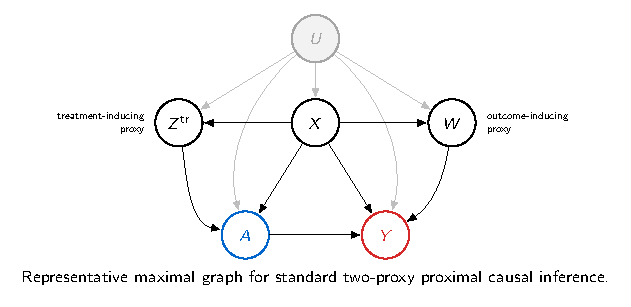
\includegraphics[width=0.46\textwidth]{../figures/2026-08-27-standard-proximal-causal-graph.pdf}}
\hfill
\subfloat[PROBE-compatible]{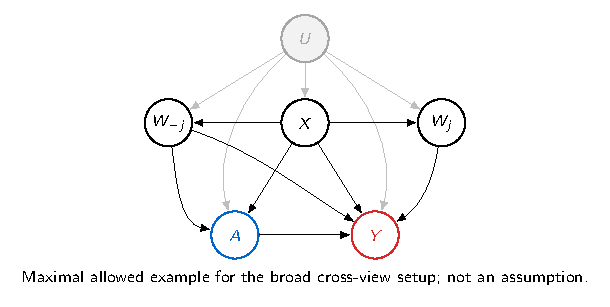
\includegraphics[width=0.46\textwidth]{../figures/2026-08-27-proximal-balancing-maximal-dependence.pdf}}
\caption{Illustrative graphs for standard proximal causal inference and PROBE. The graphs do not by themselves imply the conditional-independence, completeness, or stability assumptions.}
\label{fig:proximal-probe-graphs}
\end{figure}
\FloatBarrier

\section{Estimating Causal Effects}
\label{sec:estimation}

\subsection{Outcome-Free Representation Learning}

For a candidate map $\phi$, let $\widehat\mu_{a,z}$ be the empirical kernel mean embedding of $(X,W)$ among observations with $A=a$ and $\phi(X)=z$. Define
\begin{align}
\widehat\Delta_z(\phi)
&\triangleq
\|\widehat\mu_{1,z}-\widehat\mu_{0,z}\|_{\mathcal H_k},\\
\widehat D(\phi)
&\triangleq
\sum_z\widehat p_z(\phi)\widehat\Delta_z(\phi).
\end{align}
The ideal empirical learner returns $\widehat\phi$ satisfying
\begin{align}
\widehat D(\widehat\phi)
\le
\inf_{\phi\in\Phi}\widehat D(\phi)
+\varepsilon_{\mathrm{opt}},
\label{eq:empirical-learner}
\end{align}
where $\varepsilon_{\mathrm{opt}}$ records optimization error. Neither $Y$ nor $U$ enters this training objective. Minimum stratum mass and representation-level overlap are enforced as admissibility conditions rather than inferred from a small penalty alone.

\subsection{Cross-Fitted Algorithm}

The operational algorithm has four stages. First, split the sample into representation-training and effect-estimation folds. Second, learn $\widehat\phi$ on the training fold by minimizing an outcome-free balance objective with Adam or a finite-class search. Third, evaluate overlap and the balance discrepancy on data not used to choose the representation. Fourth, set $Z=\widehat\phi(X)$ on the effect-estimation fold and estimate the adjusted contrast. Rotating the folds and averaging estimates uses every observation while preserving the conditional fixed-representation argument.

Current neural implementations optimize differentiable soft assignments and may deploy a hard map. If $\widehat D_{\mathrm{soft}}$ is used in place of the analyzed hard-stratum objective, a valid theorem needs an explicit soft-to-hard error $\varepsilon_{\mathrm{soft}}$. The existence of such a uniform bound for the current networks is open; the manuscript will report the training surrogate and held-out hard discrepancy separately.

\subsection{AIPW Estimation for a Fixed Representation}

For fixed finite $Z$, define the nuisance functions only now:
\begin{align}
e_Z(z)&\triangleq P(A=1\mid Z=z),\\
m_a(z)&\triangleq\mathbb E(Y\mid A=a,Z=z).
\end{align}
Given cross-fitted estimates $\widehat e_Z$ and $\widehat m_a$, the augmented inverse-probability weighted estimator is
\begin{align}
\widehat\tau_{\mathrm{AIPW}}
=\frac{1}{n}\sum_{i=1}^n
\Bigg[
&\widehat m_1(Z_i)-\widehat m_0(Z_i)
+\frac{A_i\{Y_i-\widehat m_1(Z_i)\}}{\widehat e_Z(Z_i)}\\
&-\frac{(1-A_i)\{Y_i-\widehat m_0(Z_i)\}}{1-\widehat e_Z(Z_i)}
\Bigg].
\label{eq:aipw}
\end{align}
For a fixed finite representation, the corresponding influence function is
\begin{align}
\psi_\phi(O)
=
\frac{A\{Y-m_1(Z)\}}{e_Z(Z)}
-
\frac{(1-A)\{Y-m_0(Z)\}}{1-e_Z(Z)}
+m_1(Z)-m_0(Z)-\tau_\phi.
\end{align}
The stratified plug-in estimator equals \eqref{eq:aipw} when empirical cell means are used, and it is asymptotically efficient for $\tau_\phi$ in the nonparametric model for $(Z,A,Y)$. This statement is established for fixed $\phi$; a complete joint limit theory for a neural, data-selected $\widehat\phi$ remains open.

\subsection{Finite-Sample Error Decomposition}

Suppose the representation class is finite and, with probability at least $1-\delta$,
\begin{align}
\sup_{\phi\in\Phi}|\widehat D(\phi)-D(\phi)|
\le r_n(\delta).
\end{align}
For a bounded kernel and the overlap and mass constants in Section~\ref{sec:identification}, the established finite-class analysis gives
\begin{align}
r_n(\delta)
=
O\!\left(
\sqrt{\frac{\log|\Phi|+\log(1/\delta)}{n p_{\min}\eta}}
+
\sqrt{\frac{M+\log|\Phi|+\log(1/\delta)}{n}}
\right),
\label{eq:rn-rate}
\end{align}
with explicit constants available from the count, kernel-embedding, and multinomial-weight concentration steps. Combining \eqref{eq:empirical-learner} with the population certificate yields
\begin{align}
|\tau_{\widehat\phi}-\tau|
&\le
\Gamma\{\widehat D(\widehat\phi)+r_n(\delta)\},\\
|\tau_{\widehat\phi}-\tau|
&\le
\Gamma\left\{\inf_{\phi\in\Phi}D(\phi)
+2r_n(\delta)+\varepsilon_{\mathrm{opt}}\right\}.
\label{eq:oracle-bound}
\end{align}

If the effect estimator also satisfies $|\widehat\tau-\tau_{\widehat\phi}|\le\varepsilon_{\mathrm{est}}$, then
\begin{align}
\boxed{
|\widehat\tau-\tau|
\le
\varepsilon_{\mathrm{est}}
+\Gamma\{\widehat D(\widehat\phi)+r_n(\delta)\}.
}
\label{eq:finite-certificate}
\end{align}
For bounded outcomes and a fixed finite representation, $\varepsilon_{\mathrm{est}}$ has an explicit Hoeffding and multinomial bound. Equation~\eqref{eq:finite-certificate} is therefore established for enumerable classes and fixed-fold evaluation. A neural-class complexity bound, a proved $\varepsilon_{\mathrm{soft}}$, and joint inference after adaptive representation selection are explicitly open. If these pieces are supplied, the right side of \eqref{eq:oracle-bound} gains the corresponding optimization, discretization, and nuisance-estimation terms rather than changing the population target.

\section{Experiments}
\label{sec:experiments}

\subsection{Questions, Comparators, and Reporting Rules}

The experiments answer four separate questions. First, does proxy-supervised representation adjustment reduce ATE error relative to adjustment using $X$ alone? Second, do the exact-assumption designs recover the known balancing structure? Third, does the finite-state experiment verify the established certificate and its failure as the proxy channel becomes ill-posed? Fourth, does the method show a useful descriptive signal in an observational benchmark with a noisy randomized reference? We report mean absolute error, root mean squared error, paired wins, held-out discrepancy, overlap diagnostics, and Monte Carlo uncertainty. Oracle procedures that observe $U$ or the true balancing score are simulation references, not implementable competitors.

\subsection{Honest Approximate SCMs}

The primary approximate study fixes the causal order $U\to(X,W)$, $(X,U)\to A$, and $(A,X,U)\to Y$. Both SCMs use $\dim(X)=20$ and $\dim(W)=10$, with twenty independently generated data sets and nested prefixes $n\in\{100,200,500,1000,2000,5000,10000\}$. SCM1 uses linear proxy measurements and a nonlinear outcome component; SCM2 changes the structural equations to nonlinear transformations while preserving the same causal order and an informative monotone proxy channel. The proposed cross-mask method learns a representation from $X$ and all but one proxy coordinate, audits balance with the held-out coordinate, and averages over masks.

At $n=1000$, the mean absolute errors of proposed/$X$-adjustment/full-$(X,W)$/oracle-$(X,U)$ were $0.169/0.601/0.310/0.130$ in SCM1 and $0.112/0.440/0.188/0.107$ in SCM2. At $n=10000$, the corresponding proposed errors were $0.199$ and $0.134$, versus $0.588$ and $0.413$ for $X$ adjustment. These are finite-sample simulation results, not a proof of the audit-view identification theorem. The self-conditioned heuristic remained substantially biased, which is consistent with the self-conditioning warning in Section~\ref{sec:identification}.

\begin{figure}[t]
\centering
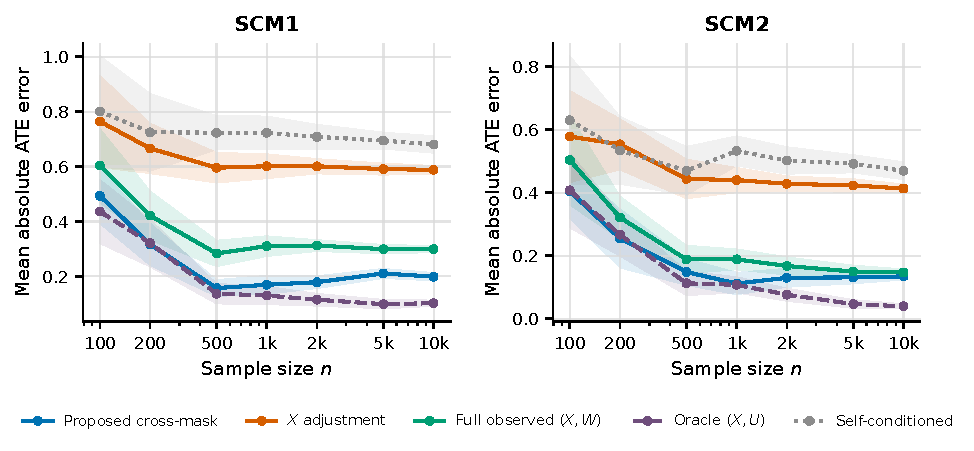
\includegraphics[width=\linewidth]{../figures/final/figure_approximate_scms.pdf}
\caption{Honest approximate SCMs. Curves show mean absolute ATE error across twenty independently generated data sets; bands are approximate $95\%$ Monte Carlo intervals for the mean. Prefixes are nested within a data set, so uncertainty is computed separately at each $n$ and is not pooled across sample sizes. The proposed cross-mask learner uses one proxy coordinate for held-out auditing and averages across masks.}
\label{fig:approximate-scms}
\end{figure}
\FloatBarrier

\subsection{Exact-Assumption Tracks A and B}

Track A uses a finite balancing score, $\dim(X)=20$, nine representation-side proxy coordinates, and one independent audit coordinate. The DGP enforces strict population overlap, exact decoding of the discrete confounding state from the representation-side view, and an injective Gaussian audit channel. At $n=10000$ over twenty replications, mean absolute error was $0.175$ for the learned audit representation, $0.433$ for $X$ adjustment, $0.186$ for direct full-observed adjustment, and $0.033$ for the oracle balancing score. The primary comparison with $X$ passed, while the prespecified secondary superiority criterion against full-observed adjustment failed.

Track B uses a continuous exact balancing score and a linear representation class matched to that score. At $n=10000$, mean absolute error was $0.0748$ for the learned representation, $0.1583$ for fitted $X$ adjustment, and $0.1342$ for fitted full-observed adjustment. The learned method beat $X$ in $20/20$ and full-observed adjustment in $19/20$ paired replications. Its mean rank-recovery Spearman correlation was $0.915$. The held-out conditional-dependence diagnostic used finite random features and is a surrogate, not an exact population KCI test; the design also covers one prespecified scalar-$U$ SCM family.

\begin{figure}[t]
\centering
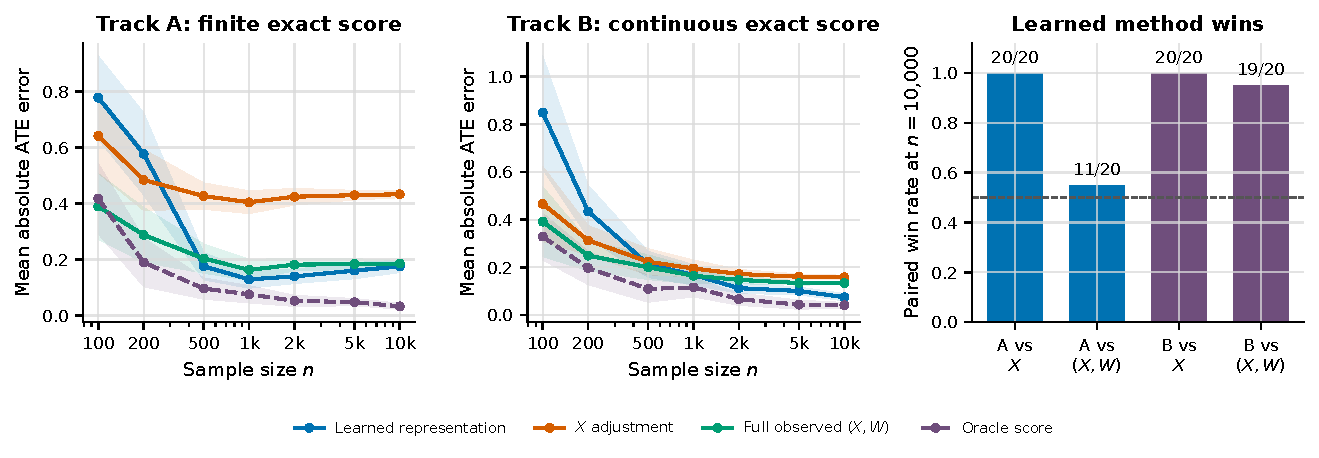
\includegraphics[width=\linewidth]{../figures/final/figure_exact_tracks.pdf}
\caption{Exact-assumption experiments. The first two panels report mean absolute ATE error with approximate $95\%$ Monte Carlo intervals over twenty replications. The third panel reports paired win rates at $n=10{,}000$, where a win means that the learned representation has smaller absolute error than the indicated comparator. Track A satisfies the primary comparison with $X$ but not the prespecified secondary superiority criterion against full observed adjustment. Track B records rank-recovery Spearman correlation $0.915$ and held-out finite-RFF conditional-dependence surrogate $0.00691$.}
\label{fig:exact-tracks}
\end{figure}
\FloatBarrier

\subsection{Finite-State Verification of the Certificate}

The population verification enumerates all $3^{10}$ candidate maps, of which $55{,}980$ satisfy the admissibility conditions. Exactly $3!=6$ maps attain exact balance, and their biases are zero to machine precision. The common certificate has zero violations over all admissible maps. As the proxy channel approaches non-injectivity, the relevant stability constant grows from $1.64$ to $48.9$ and then diverges, even while the observable discrepancy can shrink. This is the intended sensitivity behavior: a small discrepancy is informative only together with a credible stability budget. The explicit finite-sample radius is valid but conservative in this design.

\subsection{WSC Observational Benchmark}

The WSC study forms an observational subset of $1{,}105$ participants whose randomized mathematics assignment agrees with pretreatment preference, and targets the population ATE in the original $2{,}200$ randomized participants. The full randomized difference in means is $0.760$ with standard error $0.151$ and serves only as a noisy benchmark. Across ten algorithmic split repetitions on this one fixed data set, the unconstrained cross-mask estimate averaged $1.302$ with split standard deviation $0.065$ and absolute benchmark gap $0.541$, compared with gaps $2.690$ for the naive observational contrast, $1.704$ for direct $X$ adjustment, and $0.672$ for direct $(X,W)$ adjustment. The unconstrained cross-mask method is the proposed WSC method shown in Figure~\ref{fig:certificate-wsc}. Its practical-overlap gate passed $0/10$ repetitions. The benchmark therefore supplies descriptive evidence only, not a validated causal-performance claim, causal ground truth, or a test of proxy validity.

\begin{figure}[t]
\centering
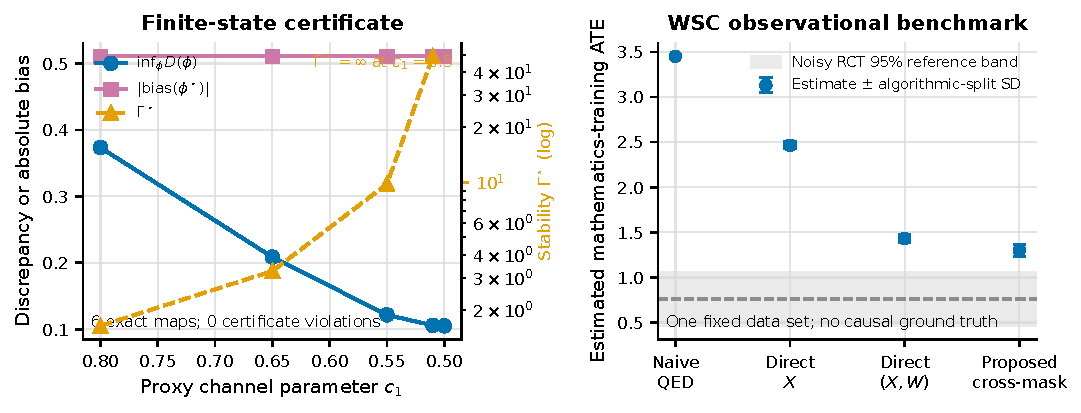
\includegraphics[width=\linewidth]{../figures/final/figure_certificate_wsc.pdf}
\caption{Certificate and observational diagnostics. Left: as the finite-state proxy channel approaches non-injectivity, the observable discrepancy decreases while realized bias remains fixed and the required stability constant diverges. Right: WSC estimates relative to the noisy randomized reference. Error bars for fitted WSC methods are standard deviations across ten algorithmic splits of one fixed data set, not Monte Carlo uncertainty. The WSC panel has no causal ground truth and reports only the unconstrained cross-mask learner as the proposed method.}
\label{fig:certificate-wsc}
\end{figure}

\clearpage

\section{Discussion and Limitations}
\label{sec:discussion}

\subsection{What the Method Delivers}

The canonical method uses a single pretreatment proxy in two roles that are available from observed data: supervising an outcome-free representation and measuring the residual imbalance of $(X,W)$ across treatment arms within that representation. Under uniform outcome-relevant stability, the product $\Gamma D(\phi)$ is a sensitivity certificate for hidden-confounding bias. This is stronger than reporting a conditional-independence test alone because it targets a causal error scale, but weaker than point identification when $D(\phi)>0$ because $\Gamma$ is not generally identified from one proxy.

\subsection{Testable and Structural Components}

Held-out joint balance, empirical overlap, and minimum stratum mass are observable properties. Proxy-channel invariance, conditional mixture injectivity, and outcome-relevant stability are structural assumptions about the full-data law. Exact balance is therefore a testable endpoint only up to sampling error, while its causal interpretation still requires structural assumptions. A large held-out discrepancy can falsify exact balance; a small test statistic cannot prove exact balance, injectivity, or stability.

\subsection{Attainability and Realized Bias}

For $Z=\phi(X)$ with finitely many strata, exact balance is attainable only on a narrow boundary characterized in Section~\ref{sec:identification}. This is a strength as a safety certificate and a limitation as a universal identification method. In the approximate regime, reducing $D(\phi)$ reduces the certified worst-case bias under a common $\Gamma$, but it need not reduce the realized bias without additional alignment conditions. Cancellation, outcome-irrelevant proxy directions, bias floors, and ill-posed channels explain why the two orderings can differ.

\subsection{Learning and Inference Gaps}

The current finite-sample theorem covers enumerable representation classes and fixed-fold evaluation. The neural experiments use soft assignments and covariance-weighted surrogate objectives that are not algebraically identical to the canonical MMD aggregation. A neural-class generalization bound, a soft-to-hard guarantee, and valid joint inference after adaptive representation selection remain open. These gaps prevent the manuscript from describing every neural result as a direct verification of the theory, even when its empirical error is lower.

\subsection{Audit Views and Practical Scope}

Cross-mask learning uses one proxy coordinate for audit and the remaining high-dimensional measurement for representation learning, then averages across audit orientations. This design blocks literal self-copying of the audited coordinate. It does not by itself establish conditional independence among proxy views, so point identification still needs a multi-view structural assumption and an audit-channel null-space condition. The WSC experiment further shows that an encouraging benchmark gap can coexist with a failed practical-overlap rule. Real-data evidence must therefore report overlap, audit discrepancies, and benchmark uncertainty without treating any one diagnostic as ground truth.

\subsection{Scope of the Contribution}

The defensible contribution is the combination of a proxy-supervised balancing representation, an observable discrepancy, an exact certification boundary, and a stability-indexed approximate guarantee. The paper does not claim that one generic proxy point-identifies the ATE, that every smaller discrepancy has smaller realized bias, or that the current neural optimizer reaches the population optimum. A systematic literature audit and broader external validation are required before any firstness or universality claim.

\section{Conclusion}
\label{sec:conclusion}

Single proxy balancing asks a deliberately limited question: what can an observed pretreatment proxy reveal about the hidden-confounding bias that remains after learning a low-dimensional adjustment representation? For the canonical construction $Z=\phi(X)$, exact observable joint balance identifies the ATE under the stated proxy conditions, while approximate balance yields the established sensitivity certificate $|\tau_\phi-\tau|\le\Gamma D(\phi)$. Empirical minimization of the discrepancy selects the smallest certified worst-case bias in the prespecified class up to generalization and optimization error. The current simulations support this mechanism in exact and approximate designs and expose important failures, including self-conditioning, ill-posed proxy channels, surrogate mismatch, and practical-overlap loss. Completing the neural learning theory and independently validating the audit-view extension are the principal steps needed to turn the present manuscript skeleton into a submission-ready paper.

\endgroup

\newpage
\bibliographystyle{apalike}
\bibliography{reference}

\clearpage
\appendix

\begingroup
\allowdisplaybreaks
\sloppy
\section{Simulation Details}
\label{app:simulations}

The existing project-local experiments will be documented by recording each data-generating process, parameter value, sample size, replication count, and random seed policy. Every manuscript figure and table will be linked to the script and machine-readable result from which it was produced.

The simulation audit will separate observed quantities from oracle quantities. In particular, any result that uses $U$ or a direction constructed from $U$ will be labeled as an oracle diagnostic and will not be presented as the output of a learnable procedure.

\section{Proof Obligations}
\label{app:proofs}

The first proof obligation is the conditioning-safety argument for $Z_j=\phi_j(X,W_{-j})$. It must show how joint latent exchangeability and separation of the held-out block remain valid after conditioning on the learned representation.

The second proof obligation is the exact bias decomposition and cross-view factorization. These results must connect the observed adjustment functional, the two treatment-arm latent laws, and the held-out distribution through one common proxy channel.

The third proof obligation is exact identification under outcome-relevant completeness. It must show that exact observed balance makes the two outcome-relevant latent averages equal without asserting equality of the full latent distributions.

The fourth proof obligation is the approximate sensitivity bound. It must show how the stability constant converts each held-out discrepancy into an outcome-relevant latent bound and how the stratum weights aggregate to $\Gamma_jD_j(\phi_j)$.

The fifth proof obligation is the finite-sample chain from uniform discrepancy concentration through empirical representation selection to honest AIPW estimation. Its final inequality must display the representation, stability, nuisance, and evaluation-sample terms separately.

\endgroup

\end{document}
